\documentclass[11pt]{amsart}
\usepackage{geometry}                % See geometry.pdf to learn the layout options. There are lots.
\geometry{letterpaper}                   % ... or a4paper or a5paper or ... 
%\geometry{landscape}                % Activate for for rotated page geometry
%\usepackage[parfill]{parskip}    % Activate to begin paragraphs with an empty line rather than an indent
\usepackage{graphicx}
\usepackage{amssymb}
\usepackage{epstopdf}
\usepackage{parskip}
\usepackage{setspace} 
\usepackage{algorithm}
\usepackage{algpseudocode}
\setlength{\parindent}{12pt}

\DeclareGraphicsRule{.tif}{png}{.png}{`convert #1 `dirname #1`/`basename #1 .tif`.png}

\title{Data Preprocessing}
\author{The Author}
%\date{}                                           % Activate to display a given date or no date
\begin{document}
\begin{spacing}{1.1}

\maketitle
%\section{}
%\subsection{}
The Dynamic Time Warping(DTW) algorithm is the one of the oldest algorithms that is used to compare and cluster sequences varying in time, length and speed. Formally, given two temporal sequences, the algorithm utilises the technique of dynamic programming to find an optimum alignment between  through the computation of local distances between the points in each sequence. The time and computational complexity of this algorithm is  \emph{O}(mn) where $m$ and $n$ denote the length of the sequences that are being compared. Thus for  high dimensional time series sequences, the time and computational costs incurred by the algorithm are quite high which  makes DTW a very unattractive choice for clustering or discovering motifs in high dimensional  data sets.  Intuitively speaking, DTW is a clustering algorithm that clusters similar patterns varying in time and speed. Another drawback for working in high-dimensional spaces is the contrast between the distances of nearest and furthest points. The distances between such points  become increasingly smaller  as the dimensionality increases. This makes it  difficult to construct meaningful cluster groups in such spaces.

To address the issue of the curse of dimensionality, DTW algorithms employ a window constraint to reduce the search space. The window constraints determine the allowable  shapes that a warping path can take. To reduce the time and computational costs incurred by the algorithm, the window size is reduced as the dimensionality of the data increases. Rigid constraints impose a more rigid alignment  that prevents an overly temporal skew between two sequences, by keeping frames of one sequence  from getting too far from the other. For clustering data sets such speech utterances, the effect produced by such global constraints is highly undesirable. If we consider two utterances of a word spoken at different time frames, the patterns can have an overly temporal askew between them as result of the different contexts in which the  words are spoken and/or as a result of  different speakers speaking the same word. Thus it is necessary to explore techniques  other than window constraints that can improve the performance of the DTW algorithm in terms of both accuracy and time. 

 Before investigating methods to improve a technique, it is highly necessary to first understand the nature of the data itself. In this chapter, I investigate data-driven preprocessing techniques  that attempt to understand the underlying intrinsic structure of the lower-dimensional space on which the  data lives. By achieving a thorough understanding of the data,we can   achieve dimensionality reduction by  isolating and identifying smaller set of new(current)  features  that are more relevant for the problem in hand. 
 
 
 There are presently two groups of preprocessing techniques commonly used to address this issue:
\begin{itemize}
\item  Feature Selection 
\item Feature Extraction
\end{itemize}
 Feature selection techniques  involve selecting only a subset of attributes from the original data.  One of the most popular approaches to feature selection is  the exploratory data analysis(EDA). EDA is an approach to data analysis that postpones the usual assumptions about what kind of model the data follows with the more direct approach of allowing the data itself to reveal its underlying structure and models. The particular techniques employed in EDA are often quite simple, consisting of various techniques of:
 
 \begin{enumerate}
\item Plotting the raw data (such as data traces, histograms, histograms, probability plots, lag plots, block plots, and Youden plots.
\item Plotting simple statistics such as mean plots, standard deviation plots, box plots, and main effects plots of the raw data.
\item Positioning such plots so as to maximize our natural pattern-recognition abilities, such as using multiple plots per page.
 \end{enumerate}
Feature extraction processes on the other hand are concerned with  a range of techniques  that apply an appropriate functional mapping to the original attributes to extract new features. The intuition behind feature extraction is that the data vectors $\{x_n\}$ typically lie close to a non- linear manifold whose intrinsic dimensionality is smaller than that of the input space as a result of strong correlations between the input features. Hence by using appropriate functional mapping, we obtain a smaller set of features that capture the intrinsic correlation between the input variable. Hence by doing so, we move from working in high dimensional spaces to working in low dimensional spaces. The choice  of appropriate functional mapping can  also improve the clustering of data as shown by figure 1:

In the rest of this chapter,  I explore a range of  feature selection and extraction methods  and investigate whether their application can improve the performance of the DTW algorithm in terms of both accuracy and time complexity.

\begin{figure}[h]
  \centering
   
     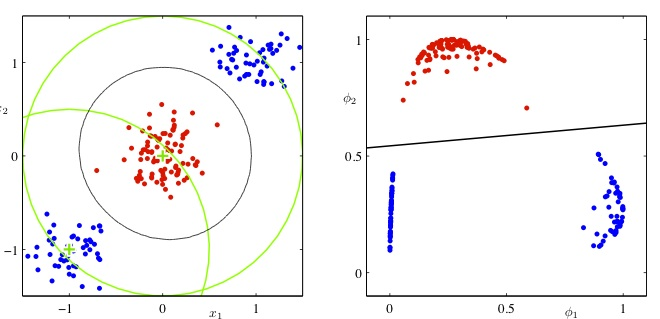
\includegraphics[scale=0.8]{featuremapping.jpg}
  \caption{The figure on the right corresponds to location of the data points in the feature space spanned by gaussian basis functions $\phi_1(x)$ and $\phi_2(x)$ }
  
\end{figure}
\newline
%The DTW algorithm combined  with the  1 nearest neighbour classifier  is a memory based algorithm. Memory-based methods involve storing the entire training set in order to make predictions for future data points. They typically require a metric to be defined that measures the similarity of any two vectors in input space, and are generally fast to �train� but slow at making predictions for test data points. The time and computational complexity associated with such methods is even higher when the dimensionality of the data points is high. Intuitively speaking, DTW is a clustering algorithm that clusters similar patterns varying in time and speed. In high- dimensional spaces, however, the contrast between the nearest and furthest points gets increasingly smaller, making it difficult to construct meaningful cluster groups. To address this issue, data dimensionality methods are used at the  preprocessing stage.
 
\section{Feature Selection}
The computational and time complexity associated with the DTW algorithm is governed by the dimensionality of the time  series. To get a feel of the data, I employed exploratory data analysis on the  isolated word utterances belonging to the test and training data sets  that I constructed from the TIDIGITS corpus. The aim here   to identify and isolate redundant features from the time series data.
 To get an idea about the structure of the data, I have studied the plots of the time series sequences along with performing auditory perception on the individual samples. Figure 2 gives the plot of raw signal corresponding to the word `8' by a speak from the \emph{boy} category. From the visual and auditory analysis, I have made the following  observations:
\begin{itemize}
\item Long durations of silence occupy the beginning and end of each utterance.   These durations of silence segments are considerably long compared to the interesting regions in the acoustic signal that actually contain information about the spoken digit .  Removing these silence segments not only  reduce the dimensionality of the time series but also results in minimal loss of information.
\item  Through auditory perception of numerous samples, I have discovered that  the recordings are highly distorted when played in matlab even when the data is scaled so that the sound is played as loud as possible without clipping. The distorted signal fails to provide any time auditory clue about  category of the speaker i.e whether the speaker belongs to \{ boy,girl, men,women\}  and the signal must be played multiple times  for its class to be correctly identified.
\end{itemize}
\begin{figure}[h!]
  \centering
   
     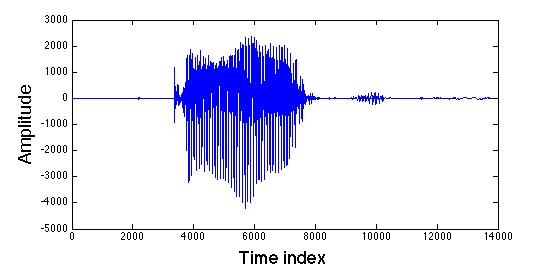
\includegraphics[scale=0.6]{Rawsample.jpg}
  \caption{`Raw 'signal}
  
\end{figure}
From  further experiments,  I have seen that if  I down-sample the utterances by $\frac{1}{2}$  which in other words means decreasing the sampling frequency by half, the resultant sampled signal is much clearer to understand. Sub-sampling  the utterances by half involves removing every other sample from the time series.  From the observation of figure 3, it can be sen that this technique  keeps the global trend of the signal intact but results in the  loss of local information. Furthermore through auditory perception of the sampled signals, I have discovered that losing some \textbf{local information} actually cleans the signal in a manner that allows the listener to identity the speaker's category and the utterance's class with ease.

With the knowledge gained from exploratory data analysis, I have constructed a  signal filter that achieves dimensionality reduction by performing feature selection. The algorithm behind the filter is as follows:

\begin{algorithm}

\begin{algorithmic}[1]
\Procedure{SignalFilter}{$signal$}\Comment{raw signal }
\State $threshold=0$
\State maxAmplitude= max(rawSignal)
 \State Adapt the threshold based on the value taken by the maximum amplitude
 \State signalSil\_R$\leftarrow$ removeSilence(rawSignal,threshold)
 \State \textbf{return} output$\leftarrow$ downsample signalSil\_R by $\frac{1}{2}$
 
 \EndProcedure
\end{algorithmic}
 \caption{SignalFilter}
\end{algorithm} 
 \begin {itemize}
 \item The algorithm removes all samples in the times series sequence whose magnitude is less than the threshold. The threshold used is an adaptive parameter. By using the information of the signal's maximum amplitude the algorithm sets the threshold accordingly. It raises the threshold for signals corresponding to speakers having a loud and deep voice is higher  and lowers the threshold for signals corresponding to speakers having as gentle and low voice.
 \end{itemize}   
  
  
 \begin{figure}[h!]
  \centering
   
     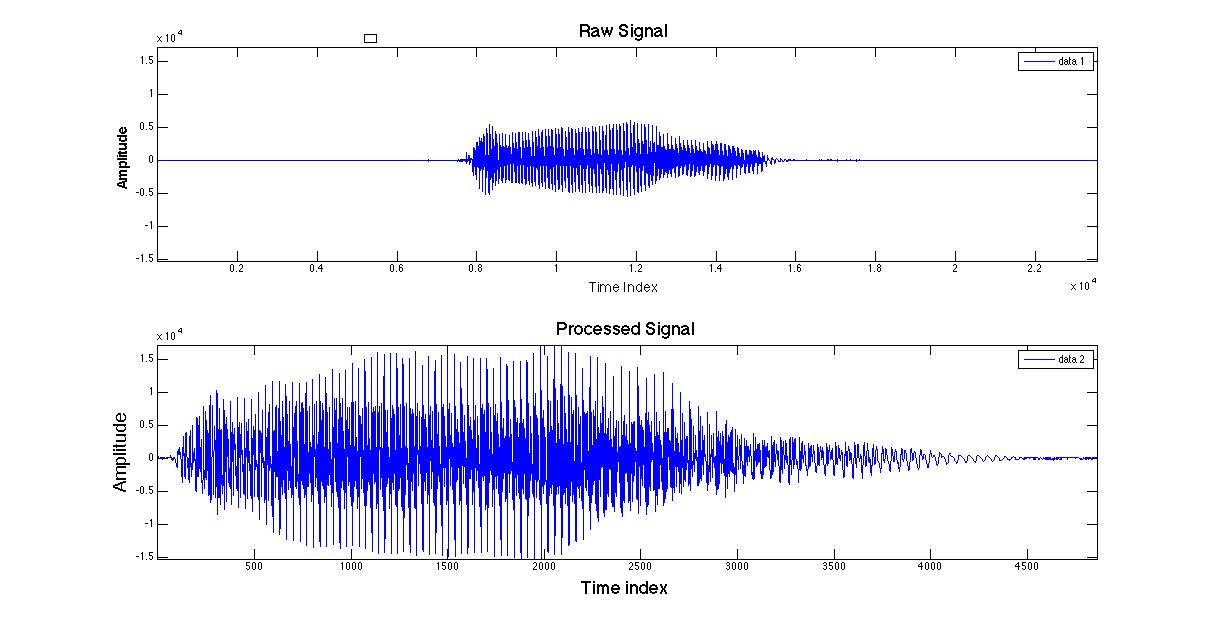
\includegraphics[scale=0.3]{Feature_selection.jpg}
  \caption{shows the raw acoustic signal corresponding to the utterances of the digit '5' alongside with the version that has its dimensionality reduced by the filter discussed above. From the comparison of the plots, it can be observed that the filter preserves the interesting patterns associated with the utterance while succeeding in reducing the dimensionality of the data.    }
  \end{figure}
  
  \newpage
 To analyse how the performance of the DTW algorithm is affected by introducing this feature selection process, I
 I ran the value-added DTW(i.e DTW using raw values)  twice  on the test data set  that I have constructed from the TIDIGITS corpus. An outline of the algorithm is given below. In the first run, I ran the algorithm using the most rigid window constraint while in the second run, I employ the feature selection process before applying the same  DTW algorithm. The results found are as follows:
 
 \newline
 \begin{algorithm}

\begin{algorithmic}[1]
\Procedure{Value-based}{$seq1,seq2$}\Comment{two raw sequences }
 \State w = max($\lceil{0.1*max(n.m)}\rceil$, abs(n-m)) \Comment{Window constraint }
 \For{i=1: to length(seq1) }\Comment{Initialise the DTW cost matrix}
 \State DTW(i,0) = $\infty$
 \EndFor
 
 \For{i=1 to length(seq2)}
 \State DTW(0,i) = $\infty$
 \EndFor
 
  \For{i=2 to length(seq1)}  
 \For{j=max(2, i-w) to min(length(seq2), i+w)} \Comment { cost(a,b)$\equiv$euclid(a,b)}
 \State DTW(i,j) = cost(seq1(i),seq2(j)) + min\{ DTW(i-1,j)+DTW(i,j-1)+DTW(i-1,j-1)\}
 \EndFor
 
 \EndFor
\State \texbf{return}  result = $\frac{\mbox{DTW(n,m))}}{nm}$ \Comment{n=length(seq1), m=length(seq2)}

\EndProcedure} 
\end{algorithmic}
\caption{Value-Based DTW}
\end{algorithm}
 

\end{spacing}
\end{document}  